% CS615 Aspects of System Administration
% Author: Jan Schaumann <jschauma@netmeister.org>
% $Id: slides.tex,v 1.6 2006/03/07 13:55:55 jschauma Exp $

\documentclass[xga]{xdvislides}
\usepackage[landscape]{geometry}
\usepackage{graphics}
\usepackage{graphicx}
\usepackage{colordvi}

\begin{document}
\setfontphv

%%% Headers and footers
\lhead{\slidetitle}                               % default:\lhead{\slidetitle}
\chead{CS615 - Aspects of System Administration}% default:\chead{\relax}
\rhead{Slide \thepage}                       % default:\rhead{\sectiontitle}
\lfoot{\Gray{DNS; HTTP}}% default:\lfoot{\slideauthor}
\cfoot{\relax}                               % default:\cfoot{\relax}
\rfoot{\Gray{\today}}

\newcommand{\smallish}{\fontsize{15}{20}\selectfont}

\vspace*{\fill}
\begin{center}
	\Hugesize
		CS615 - Aspects of System Administration\\ [1em]
		DNS; HTTP\\ [1em]
	\hspace*{5mm}\blueline\\ [1em]
	\Normalsize
		Department of Computer Science\\
		Stevens Institute of Technology\\
		Jan Schaumann\\
		\verb+jschauma@stevens-tech.edu+
		\verb+https://www.cs.stevens.edu/~jschauma/615/+
\end{center}
\vspace*{\fill}

\subsection{Current Events} \begin{center} 1.35 Tb/s
DDoS on GitHub \\ \vspace{.25in}
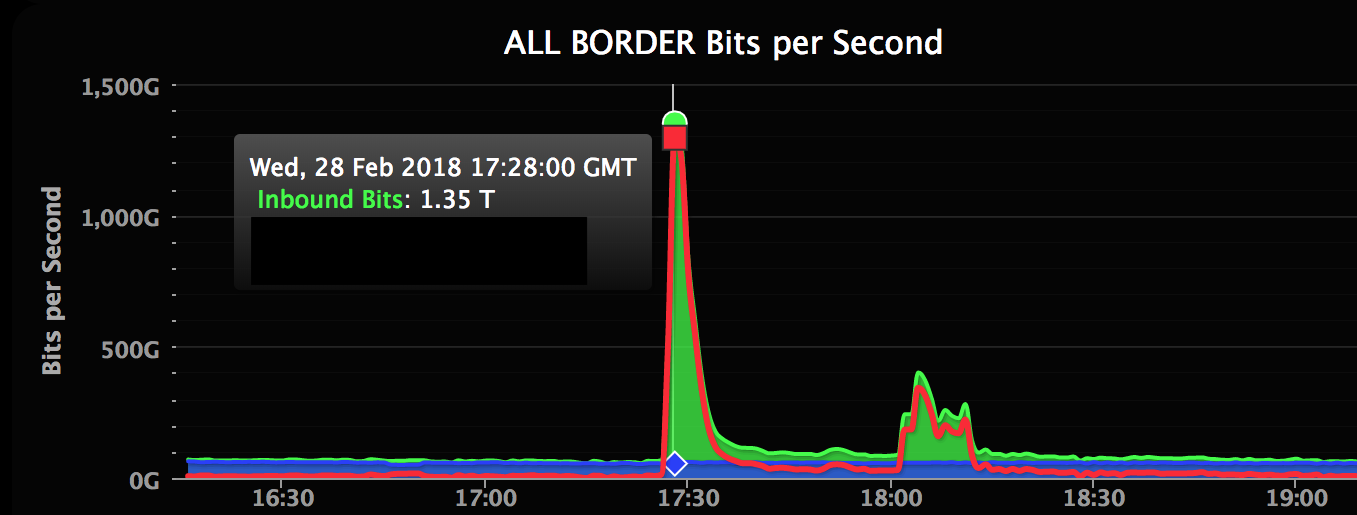
\includegraphics[scale=0.4]{pics/github-ddos.eps} \\
\vspace{.25in} {\tt
https://www.wired.com/story/github-ddos-memcached/} \\
{\tt
https://githubengineering.com/ddos-incident-report/}
\end{center}

\subsection{Current Events}

Reminder: The Cloud is just other people's computers.
\\
\begin{center}

\includegraphics[scale=1.0]{pics/clown-computing.eps} \\
\end{center}

AWS US-EAST-1 Region downtime leads to outages and
connectivity degradation for Atlassian's Bitbucket,
Confluence, and Jira, GitHub, MongoDB, NewVoiceMedia,
Slack, Twilio, Zillow. \\

{\tt https://is.gd/gvI38X}

\subsection{Keeping track...}

\begin{itemize}
	\item {\tt http://www.devopsweekly.com/}
	\item {\tt https://sreweekly.com/}
	\item {\tt https://www.nanog.org/}
	\item {\tt https://puck.nether.net/mailman/listinfo/outages}
\end{itemize}

\subsection{In the beginning...}
\vspace*{\fill}
\begin{center}
	\includegraphics[scale=0.8]{pics/2computers.eps} \\
\end{center}
\vspace*{\fill}

\subsection{In the beginning...}
\vspace*{\fill}
\begin{center}
	\includegraphics[scale=0.8]{pics/2computers-nic.eps} \\
\end{center}
\vspace*{\fill}

\subsection{In the beginning...}
\vspace*{\fill}
\begin{center}
	\includegraphics[scale=0.8]{pics/3computers.eps} \\
\end{center}
\vspace*{\fill}

\subsection{In the beginning...}
\vspace*{\fill}
\begin{center}
	\includegraphics[scale=0.8]{pics/3computers-1.eps} \\
\end{center}
\vspace*{\fill}

\subsection{In the beginning...}
\vspace*{\fill}
\begin{center}
	\includegraphics[scale=0.8]{pics/3computers-2.eps} \\
\end{center}
\vspace*{\fill}

\subsection{In the beginning...}
\vspace*{\fill}
\begin{center}
	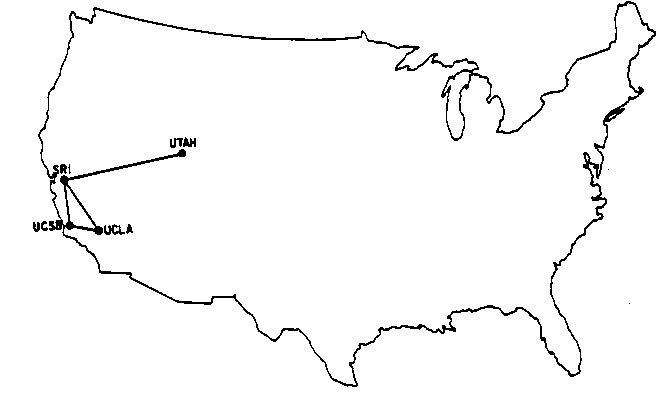
\includegraphics[scale=0.8]{pics/arpanet1.eps} \\
	{\tt https://is.gd/DdPNCo} \\
\end{center}
\vspace*{\fill}


\subsection{In the beginning...}
\begin{verbatim}
# Host Database
# This file should contain the addresses and aliases
# for local hosts that share this file.
#
127.0.0.1               localhost localhost.
#
# RFC 1918 specifies that these networks are "internal".
# 10.0.0.0      10.255.255.255
# 172.16.0.0    172.31.255.255
# 192.168.0.0   192.168.255.255
10.0.0.1	UCLA-TEST
10.0.0.2	SRI-SPRM
10.0.0.4	UTAH-CS
\end{verbatim}


\subsection{But then...}
\vspace*{\fill}
\begin{center}
	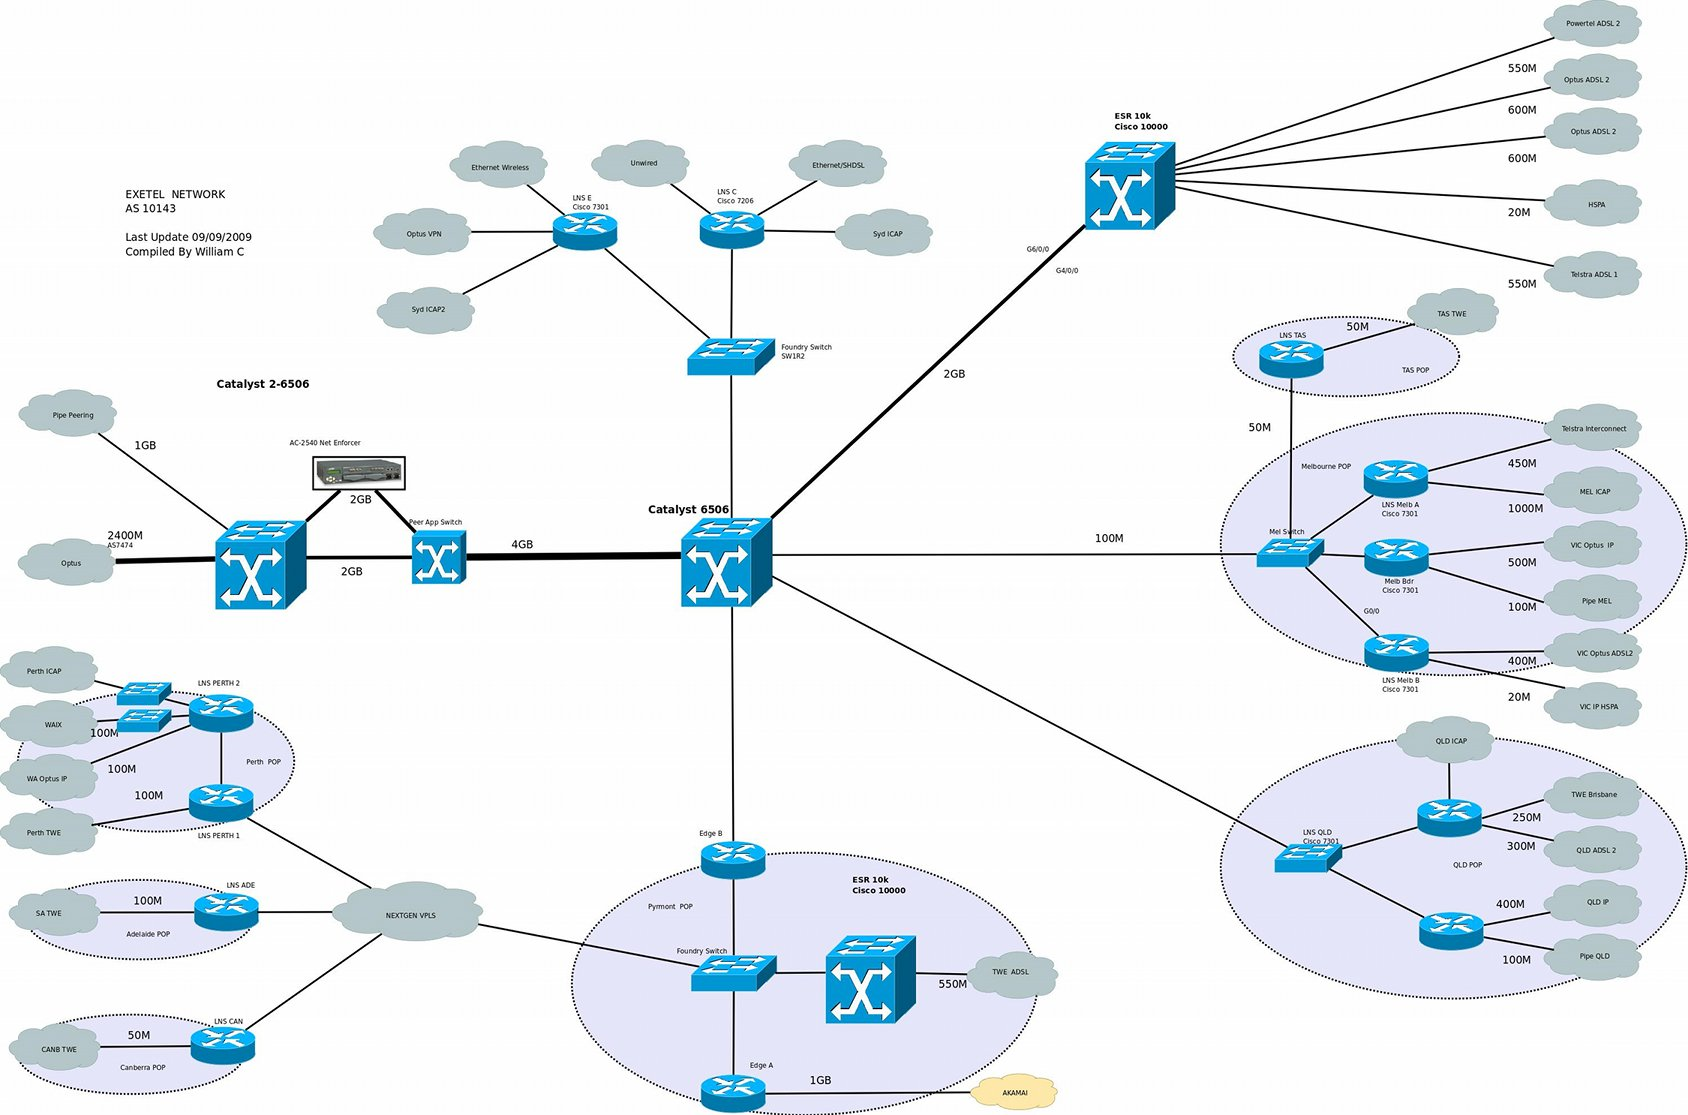
\includegraphics[scale=0.3]{pics/routed.eps} \\
\end{center}
\vspace*{\fill}

\subsection{The Domain Name System}
\vspace{.5in}
\begin{center}
	\Huge
	Computers like numbers. \\
\vspace{.5in}
\begin{verbatim}
         10011011111101100101100110011111
\end{verbatim}
\end{center}
\Normalsize

\subsection{The Domain Name System}
\vspace{.5in}
\begin{center}
	\Huge
	Computers like numbers. \\
\vspace{.5in}
\begin{verbatim}
      10011011  11110110  01011001  10011111

        155   .   246   .    89   .   159
\end{verbatim}
\end{center}
\Normalsize

\subsection{The Domain Name System}
\vspace{.5in}
\begin{center}
	\Huge
	People like names. \\
\vspace{.5in}
\verb+ash.cs.stevens-tech.edu+
\end{center}
\Normalsize


\subsection{The Domain Name System}
\vspace*{\fill}
\begin{center}
	
\includegraphics[scale=0.6]{pics/phonebook.eps}
\end{center}
\vspace*{\fill}

\subsection{The New Phonebook is here!}
\vspace*{\fill}
\begin{center}
	\verb+https://is.gd/XXp2sC+ \\
	\addvspace{.5in}
	\verb+wget -q -O - https://is.gd/XXp2sC | grep -c "^HOST"+
\end{center}
\vspace*{\fill}

\subsection{DNS: A distributed database}
\vspace*{\fill}
\begin{center}
	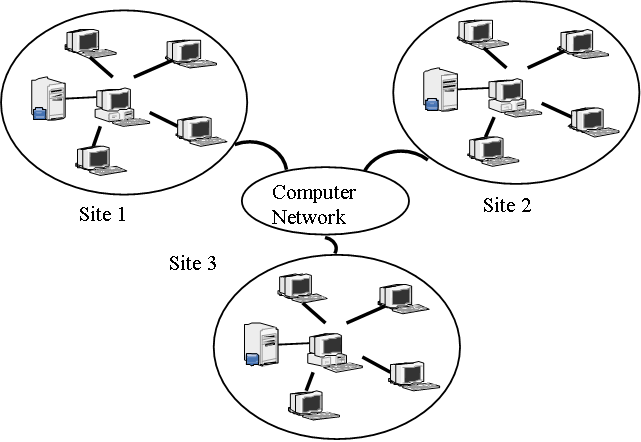
\includegraphics[scale=0.75]{pics/distributed-database.eps}
\end{center}
\vspace*{\fill}

\subsection{The Domain Name Space}
\vspace{.5in}
\begin{center}
	\Huge
	The domain name space consists of a tree of {\em domain} names.
\end{center}
\Normalsize

\subsection{DNS: A hierarchical system}
\vspace*{\fill}
\begin{center}
	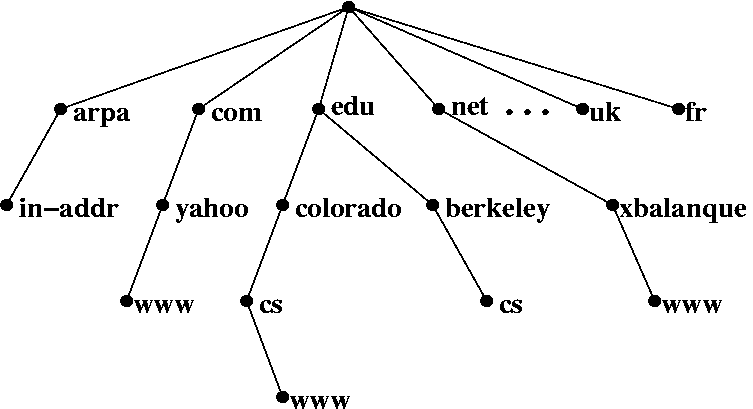
\includegraphics[scale=0.75]{pics/hierarchical-dns.eps}
\end{center}
\vspace*{\fill}

\subsection{The Domain Name Space}
\vspace{.5in}
\begin{center}
	\Huge
	The domain name space consists of a tree of {\em domain} names. \\
	\vspace{.5in}
	A subtree divides into {\em zones}.
\end{center}
\Normalsize

\subsection{The Domain Name Space}
\vspace{.5in}
\begin{center}
	\Huge
	The domain name space consists of a tree of {\em domain} names. \\
	\vspace{.5in}
	A subtree divides into {\em zones}. \\
	\vspace{.5in}
	Each node may contain {\em resource records}.
\end{center}
\Normalsize

\subsection{The Domain Name Space}
\vspace*{\fill}
\begin{center}
	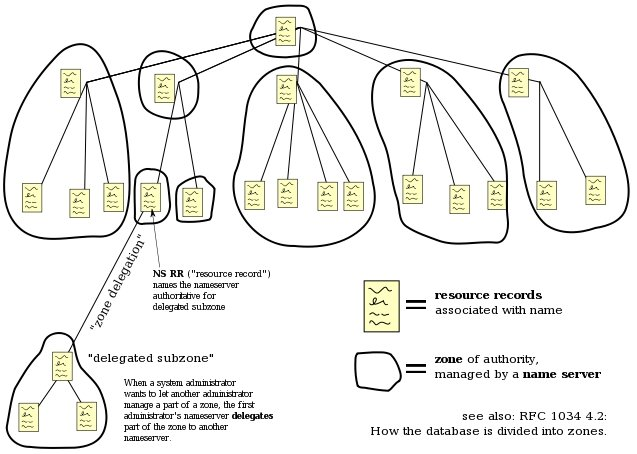
\includegraphics[scale=0.74]{pics/dns-space.eps}
\end{center}
\vspace*{\fill}

\subsection{Domain Names}
\vspace{.5in}
\begin{center}
	\Huge
	\verb+ash.cs.stevens-tech.edu+ \\
	\vspace{.5in}
	Domain Names are read from right to left and components separated by a ``\verb+.+''.
\end{center}
\Normalsize

\subsection{Domain Names}
\vspace{.5in}
\begin{center}
	\Huge
	\verb+ash.cs.stevens-tech.edu.+ \\
	\vspace{.5in}
	The {\em root} is known as ``\verb+.+'', but is usually left out.
\end{center}
\Normalsize

\subsection{Domain Names}
\vspace{.5in}
\begin{center}
	\Huge
	\verb+ash.cs.stevens-tech.+{\bf edu}\verb+.+ \\
	\vspace{.5in}
	There is a small number of {\em top level domains}.
\end{center}
\Normalsize

\subsection{Domain Names}
\vspace{.5in}
\begin{center}
	\Huge
	\verb+ash.cs.stevens-tech.+{\bf edu}\verb+.+ \\
	\vspace{.5in}
	There is a number of {\em top level domains}. \\
	\vspace{.5in}
	\Normalsize
	\begin{verbatim}
wget -O - ftp://rs.internic.net/domain/root.zone | \
        grep "IN<tab>*NS<tab>" | awk '{print $1}' | sort -u | wc -l
\end{verbatim}
	\vspace{.25in}
	\verb+https://data.iana.org/TLD/tlds-alpha-by-domain.txt+ \\
	\verb+https://en.wikipedia.org/wiki/List_of_Internet_top-level_domains+
\end{center}
\Normalsize


\subsection{Domain Names}
\vspace{.5in}
\begin{center}
	\Huge
	\verb+ash.cs.+{\bf stevens-tech}\verb+.edu.+ \\
	\vspace{.5in}
	Each {\em domain} can be divided into any number of {\em sub domains}.
\end{center}
\Normalsize

\subsection{Domain Names}
\vspace{.5in}
\begin{center}
	\Huge
	\verb+ash.+{\bf cs}\verb+.stevens-tech.edu.+ \\
	\vspace{.5in}
	Each {\em domain} can be divided into any number of {\em sub domains}.
\end{center}
\Normalsize

\subsection{Domain Names}
\vspace{.5in}
\begin{center}
	\Huge
	{\bf ash}\verb+.cs.stevens-tech.edu.+ \\
	\vspace{.5in}
	The left-most component of a domain name may be a {\em hostname}.
\end{center}
\Normalsize

\subsection{Fully Qualified Domain Names}
\vspace{.5in}
\begin{center}
	\Huge
	\verb+ash.cs.stevens-tech.edu.+ \\
	\vspace{.5in}
	A {\em hostname} with a domain name is known as a {\em FQDN}.
\end{center}
\Normalsize

\subsection{The Original IANA}
\vspace*{\fill}
\begin{center}
	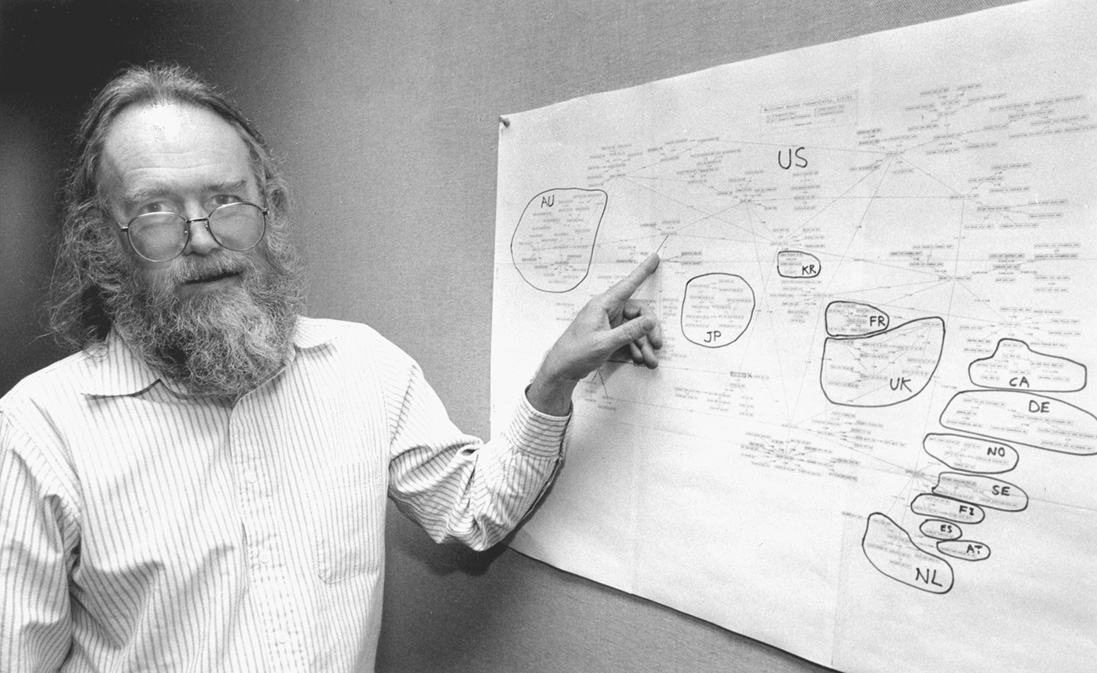
\includegraphics[scale=1.25]{pics/postel.eps}
\end{center}
\vspace*{\fill}

\subsection{NIC and Network Solutions}
Before the DNS, the Network Information Center (NIC)
at Stanford Research Institute (SRI) allocated domain
names. IANA (effectively: Jon Postel) assigned, NIC
published.  \\

{\tt https://www.internic.net} \\

In 1991, this was contracted out to Network Solutions,
Inc. (NSI), which held the monopoly on DNS
registrations (within .com, .org, .mil, .gov, .edu, and
.net) until around 1998. \\


\subsection{Registries}
IANA manages the root zone (.), arpa.; gTLD registries
handle gTLDs, ccTLD registries handle ccTLDs.  ICANN
accredits {\em domain name registries}. \\

Registries
\begin{itemize}
	\item may function as a Domain Name Registrar
	\item may delegate Domain Name registration
	\item control policies of allocations
	\item can (and do) censor, revoke, change, ... entries (e.g. {\tt vb.ly})
\end{itemize}

\vspace{.5in}
The domain name space is a tree; if you control one
node, you control all the branches and subtrees.

\subsection{DNS servers come in two flavors}
\vspace*{\fill}
\begin{center}
	\begin{tabular}{ c c c }
	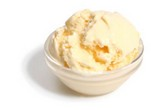
\includegraphics[scale=1.5]{pics/vanilla.eps} & \hspace{.5in} & 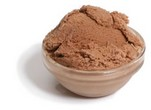
\includegraphics[scale=1.5]{pics/chocolate.eps} \\
	\hspace{.3in} \Huge Authoritative & & \hspace{.3in} \Huge Recursive \\
	\hspace{.3in} \Huge Nameservers & & \hspace{.3in} \Huge Nameservers \\
	\end{tabular}
\end{center}
\vspace*{\fill}

\subsection{Hostname resolution}
Resolution on a recursive nameserver (aka {\em resolver}) involves a number of queries:
\vspace{.5in}
\begin{verbatim}
$ nslookup ash.cs.stevens-tech.edu
Server:         127.0.0.1
Address:        127.0.0.1#53

Non-authoritative answer:
Name:   ash.cs.stevens-tech.edu
Address: 155.246.89.159

$
\end{verbatim}

\subsection{Hostname resolution}
Resolution on a {\em resolver} involves a number of queries:
\begin{verbatim}
IP panix.netmeister.org.62105 > i.root-servers.net.domain:
        11585 [1au] A? ash.cs.stevens-tech.edu. (52)
IP i.root-servers.net.domain > panix.netmeister.org.62105:
        11585- 0/8/8 (494)
IP panix.netmeister.org.53168 > a.gtld-servers.net.domain:
        46575 [1au] A? ash.cs.stevens-tech.edu. (52)
IP a.gtld-servers.net.domain > panix.netmeister.org.53168:
        46575- 0/6/3 (609)
IP panix.netmeister.org.41071 > nrac.stevens-tech.edu.domain:
        24322 [1au] A? ash.cs.stevens-tech.edu. (52)
IP nrac.stevens-tech.edu.domain > panix.netmeister.org.41071:
        24322*- 1/2/3 A[|domain]
\end{verbatim}
\Normalsize

\subsection{Hostname resolution}
Resolution on a {\em resolver} involves a number of queries:
\begin{verbatim}
$ host -t ns .
. name server I.ROOT-SERVERS.NET.
. name server D.ROOT-SERVERS.NET.
. name server C.ROOT-SERVERS.NET.
. name server M.ROOT-SERVERS.NET.
. name server F.ROOT-SERVERS.NET.
. name server A.ROOT-SERVERS.NET.
. name server E.ROOT-SERVERS.NET.
. name server L.ROOT-SERVERS.NET.
. name server H.ROOT-SERVERS.NET.
. name server J.ROOT-SERVERS.NET.
. name server B.ROOT-SERVERS.NET.
. name server G.ROOT-SERVERS.NET.
. name server K.ROOT-SERVERS.NET.
$
\end{verbatim}

\subsection{Hostname resolution}
Resolution on a {\em resolver} involves a number of queries:
\begin{verbatim}
$ dig -t ns edu.
[...]
;; ANSWER SECTION:
edu.                    172800  IN      NS      l.edu-servers.net.
edu.                    172800  IN      NS      f.edu-servers.net.
edu.                    172800  IN      NS      c.edu-servers.net.
edu.                    172800  IN      NS      g.edu-servers.net.
edu.                    172800  IN      NS      a.edu-servers.net.
edu.                    172800  IN      NS      d.edu-servers.net.

;; ADDITIONAL SECTION:
c.edu-servers.net.      36626   IN      A       192.26.92.30
d.edu-servers.net.      13274   IN      A       192.31.80.30
l.edu-servers.net.      36626   IN      A       192.41.162.30
[...]
$
\end{verbatim}
\Normalsize

\subsection{Hostname resolution}
Resolution on a {\em resolver} involves a number of queries:
\begin{verbatim}
$ dig @c.edu-servers.net -t ns stevens.edu.
[...]
;; AUTHORITY SECTION:
stevens.edu.            172800  IN      NS      nrac.stevens-tech.edu.
stevens.edu.            172800  IN      NS      sitult.stevens-tech.edu.

;; ADDITIONAL SECTION:
nrac.stevens-tech.edu.  172800  IN      A       155.246.1.21
sitult.stevens-tech.edu. 172800 IN      A       155.246.1.20
[...]
$
\end{verbatim}

\subsection{Hostname resolution}
\vspace*{\fill}
\begin{center}
	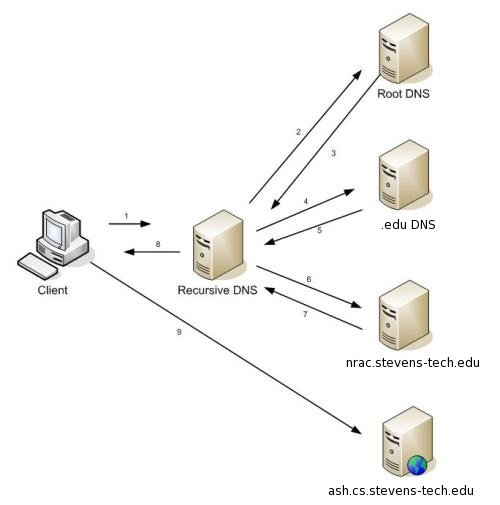
\includegraphics[scale=0.9]{pics/resolution.eps}
\end{center}
\vspace*{\fill}


\subsection{Hostname resolution}
Resolution on a {\em resolver} involves a number of queries:
\begin{verbatim}
$ nslookup ash.cs.stevens-tech.edu
Server:         127.0.0.1
Address:        127.0.0.1#53

Non-authoritative answer:
Name:   ash.cs.stevens-tech.edu
Address: 155.246.89.159

$
\end{verbatim}

\subsection{Hostname resolution}
\vspace*{\fill}
\begin{center}
	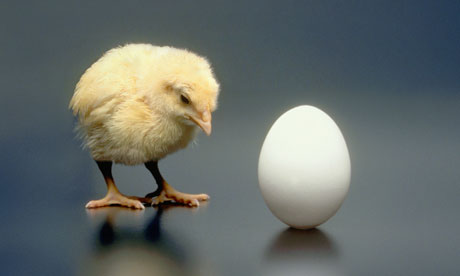
\includegraphics[scale=0.4]{pics/chicken-egg.eps} \\
	\vspace*{\fill}
\end{center}

\subsection{Hostname resolution}
\vspace*{\fill}
\begin{center}
	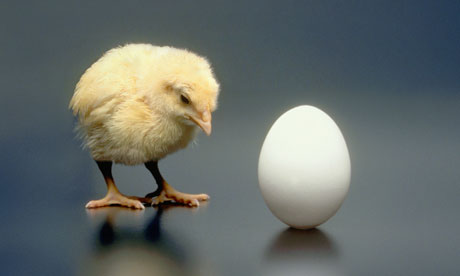
\includegraphics[scale=0.4]{pics/chicken-egg.eps} \\
	\addvspace{.2in}
	\verb+$ ftp -o - ftp.internic.net:/domain/db.cache | more+ \\
	\verb+https://www.internic.net/zones/named.root+
	\vspace*{\fill}
\end{center}

\subsection{Operation Global Blackout}
\vspace*{\fill}
\begin{center}
	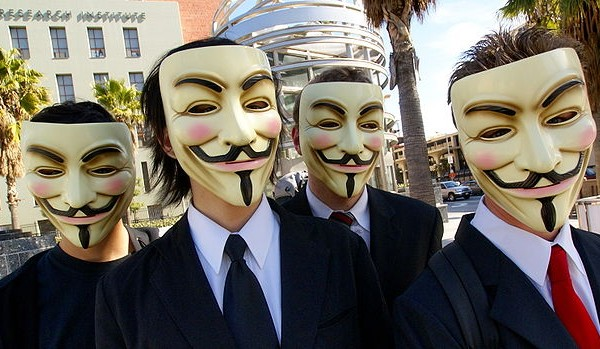
\includegraphics[scale=0.8]{pics/anonymous.eps} \\
	\addvspace{.2in}
	\verb+https://pastebin.com/XZ3EGsbc+ \\
	\addvspace{.1in}
\end{center}
\vspace*{\fill}

\subsection{DNS: A distributed system}
\vspace{.5in}
\begin{center}
	\Huge
	There are 13 \verb+root+ servers. \\
\end{center}
\Normalsize

\subsection{DNS: A distributed system}
\vspace{.5in}
\begin{center}
	\Huge
	There are 13 \verb+root+ servers. \\
	\vspace{.5in}
	Except... there are more.
\end{center}
\Normalsize

\subsection{DNS: A distributed system}
\vspace{.5in}
\begin{center}
	\Huge
	There are 13 \verb+root+ {\em authorities}. \\
\end{center}
\Normalsize

\subsection{DNS: A distributed system}
\vspace{.5in}
\begin{center}
	\Huge
	There are 13 \verb+root server+ {\em addresses}. \\
\end{center}
\Normalsize

\subsection{DNS: A distributed system}
\vspace{.5in}
\begin{center}
	\Huge
	There are hundreds of \verb+root+ servers. \\
\end{center}
\Normalsize

\subsection{DNS: A distributed system}
\vspace*{\fill}
\begin{center}
	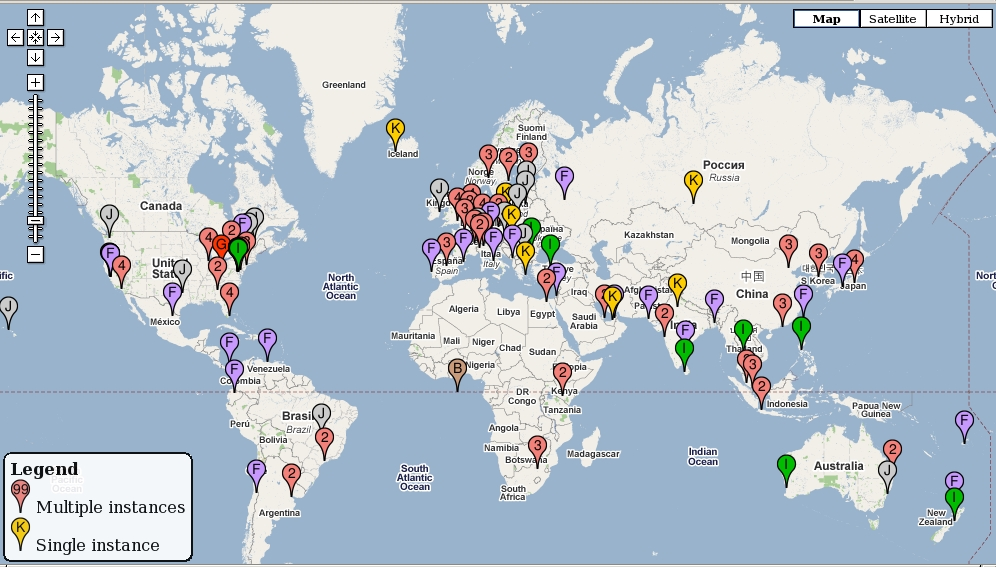
\includegraphics[scale=0.5]{pics/root-servers.eps}
\end{center}
\vspace*{\fill}
See e.g.: {\tt https://e.root-servers.org/}

\subsection{Operation Global Blackout}
\vspace*{\fill}
\begin{center}
	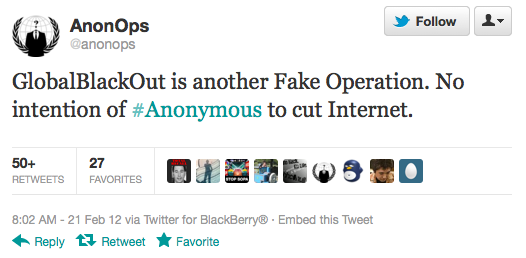
\includegraphics[scale=0.8]{pics/anonymous-tweet.eps} \\
\end{center}
\vspace*{\fill}


\subsection{DNS: A distributed database}
\vspace*{\fill}
\begin{center}
	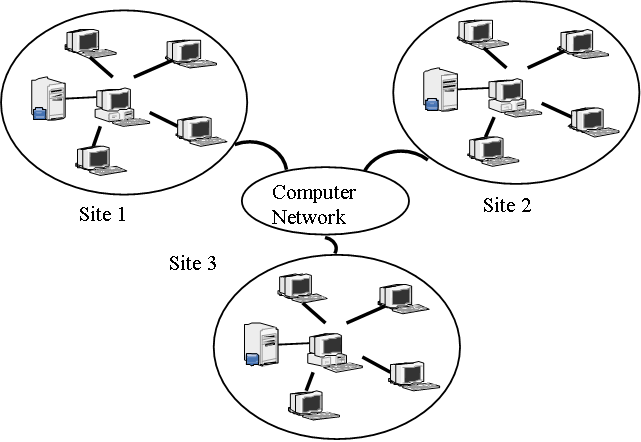
\includegraphics[scale=0.75]{pics/distributed-database.eps}
\end{center}
\vspace*{\fill}


\subsection{DNS Resource Records}
More than just {\tt A} and {\tt AAAA}:
\begin{itemize}
	\item {\em CAA} -- certificate authority authorization
	\item {\em CNAME} -- the canonical name for an alias
	\item {\em MX} -- mail exchange
	\item {\em NS} -- an authoritative name server
	\item {\em SOA} -- marks the start of a zone of authority
	\item {\em SRV} -- service locator (e.g. for kerberos)
	\item {\em PTR} -- a domain name pointer
	\item {\em TXT} text strings
	\item ...
\end{itemize}

\subsection{DNS Resource Records}
You've all seen PTR records:
\\

\begin{verbatim}
$ host ash.cs.stevens-tech.edu
ash.cs.stevens-tech.edu has address 155.246.89.159
ash.cs.stevens-tech.edu mail is handled by 0 guinness.cs.stevens-tech.edu.
$ host 155.246.89.159
159.89.246.155.in-addr.arpa domain name pointer ash.cs.stevens-tech.edu.
$ 
\end{verbatim}

Stevens doesn't have write access to the {\tt
in-addr.arpa} domain.  How does this work?
 
\subsection{Creative uses of DNS Resource Records}
\begin{itemize}
	\item identifying sources of SPAM (via e.g. an RBL)
	\item detect email spoofing (via e.g. SPF)
	\item find out if the internet is on fire: \\
		\verb|dig +short txt istheinternetonfire.com|
	\item find ASN numbers by IP addresses: \\
		\verb|dig +short 159.89.246.155.origin.asn.cymru.com TXT|
	\item check a resolver's source port randomization (to help
		mitigate DNS Cache Poisoning attacks): \\
		\verb|dig +short porttest.dns-oarc.net TXT|
	\item using DNS to publish SSH key fingerprints (RFC4255,
ssh\_config(5) \verb+VerifyHostKeyDNS+; for best results combine with DNSSEC)
\end{itemize}

\newpage
\vspace*{\fill}
\begin{center}
    \Hugesize
        Hooray! \\ [1em]
    \hspace*{5mm}
    \blueline\\
    \hspace*{5mm}\\
        5 Minute Break
\end{center}
\vspace*{\fill}

\newpage
\vspace*{\fill}
\begin{center}
	\Hugesize
		Hypertext Transfer Protocol\\ [1em]
	\hspace*{5mm}
	\blueline\\
	\hspace*{5mm}\\
		Today's Universal Internet Pipe
\end{center}
\vspace*{\fill}

%\subsection{Set up an HTTP server.}
%
%\vspace*{\fill}
%Start an EC2 instance and set up an HTTP server to listen on port 8080.
%Add a simple index.html file containing your username.
%
%When done, paste the full URL (ie http:///) into the class IRC channel
%\#cs615asa.
%
%{\tt https://webchat.freenode.net/}
%\vspace*{\fill}

\subsection{HTTP: Hypertext}
\vspace{.5in}
\begin{center}
	\Huge
	W W W
	\\
\vspace{.5in}
	{\em ``The World Wide Web is the only thing I know of whose shortened form
	takes three times longer to say than what it's short for.'' -- Douglas Adams}
\end{center}
\Normalsize


\subsection{HTTP: Hypertext}
\begin{center}
	\includegraphics[scale=0.9]{pics/http-proposal-detail.eps} \\
	\vspace{.5in}
	\verb+https://is.gd/JnZaN6+
\end{center}

\subsection{HTTP}
\vspace{.5in}
\begin{center}
	\Huge
	Hypertext Transfer Protocol
	\\
	\vspace{.5in}
	RFC2616
\end{center}
\Normalsize

\subsection{HTTP}
\vspace{.5in}
\begin{center}
	\Huge
	HTTP is a request/response protocol.
\end{center}
\Normalsize

\subsection{The Hypertext Transfer Protocol}
HTTP is a request/response protocol:
\begin{enumerate}
	\item client sends a request to the server
	\item server responds
\end{enumerate}

\subsection{The Hypertext Transfer Protocol}
HTTP is a request/response protocol:
\begin{enumerate}
	\item client sends a request to the server
		\begin{itemize}
			\item request method
			\item URI
			\item protocol version
			\item request modifiers
			\item client information
		\end{itemize}
	\item server responds
\end{enumerate}

\subsection{HTTP: A client request}
\vspace*{.5in}
\\
\Hugesize
\begin{center}
\begin{verbatim}
$ telnet www.google.com 80
Trying 173.194.75.147...
Connected to www.google.com.
Escape character is '^]'.
GET / HTTP/1.0
\end{verbatim}
\end{center}
\Normalsize
\vspace*{\fill}


\subsection{The Hypertext Transfer Protocol}
HTTP is a request/response protocol:
\begin{enumerate}
	\item client sends a request to the server
		\begin{itemize}
			\item request method
			\item URI
			\item protocol version
			\item request modifiers
			\item client information
		\end{itemize}
	\item server responds
		\begin{itemize}
			\item status line (including success or error code)
			\item server information
			\item entity metainformation
			\item content
		\end{itemize}
\end{enumerate}

\subsection{HTTP: a server response}
%\smallish
\begin{verbatim}
HTTP/1.0 200 OK
Date: Sun, 31 Mar 2013 01:54:40 GMT
Set-Cookie: PREF=ID=c5eb56d629b347cc:FF=0:TM=1364694880:LM=1364694880:
S=sIdRFdxV9YvtQOlG; expires=Tue, 31-Mar-2015 01:54:40 GMT; path=/;
domain=.google.com
Set-Cookie: NID=67=hvBnOob2NoZW4haTJVfajbcyn_jips50lKRe-8nawzdCZ6AukNR
_s8CNHD6ZA-Z2721nA3TpLrNXt-2zyIui23j4kdsdF8Gg--PmGsMOJ3Jv5frEzQG1elHJv92HL-w2;
expires=Mon, 30-Sep-2013 01:54:40 GMT; path=/; domain=.google.com; HttpOnly
Server: gws

<!doctype html><html itemscope="itemscope" itemtype="http://schema.org/WebPage">
<head><meta content="Search the...

\end{verbatim}
%\Normalsize

\subsection{The Hypertext Transfer Protocol}
Server status codes:
\begin{itemize}
	\item {\bf 1xx} -- Informational; Request received, continuing process
	\item {\bf 2xx} -- Success; The action was successfully received,
        understood, and accepted
	\item {\bf 3xx} -- Redirection; Further action must be taken in order to
        complete the request
	\item {\bf 4xx} -- Client Error; The request contains bad syntax or
		cannot be fulfilled
	\item {\bf 5xx} -- Server Error; The server failed to fulfill an
		apparently valid request
\end{itemize}

\subsection{HTTP: A client request}
\smallish
\begin{verbatim}
$ telnet www.cs.stevens.edu 80
Trying 155.246.89.84...
Connected to www.cs.stevens-tech.edu.
Ecape character is '^]'.
GET / HTTP/1.0

HTTP/1.1 301 Moved Permanently
Date: Mon, 05 Mar 2018 20:41:06 GMT
Server: Apache
Location: https://www.cs.stevens.edu/
Vary: Accept-Encoding
Content-Length: 235
Connection: close
Content-Type: text/html; charset=iso-8859-1
\end{verbatim}
\Normalsize

\subsection{HTTP: A client request}
\smallish
\begin{verbatim}
$ printf "HEAD / HTTP/1.1\r\nHost: www.cs.stevens.edu\r\n\r\n" |
        openssl s_client -quiet -ign_eof -connect www.cs.stevens.edu:443 2>/dev/null

HTTP/1.1 302 Found
Date: Mon, 05 Mar 2018 20:53:38 GMT
Server: Apache
Location: https://www.stevens.edu/ses/cs
Vary: Accept-Encoding
Content-Type: text/html; charset=iso-8859-1
\end{verbatim}
\Normalsize

\subsection{HTTP: A client request}
\smallish
\begin{verbatim}
$ printf "HEAD /ses/cs HTTP/1.1\r\nHost: www.stevens.edu\r\n\r\n" |
        openssl s_client -quiet -ign_eof -connect www.stevens.edu:443 2>/dev/null

HTTP/1.1 301 Moved Permanently
Date: Mon, 05 Mar 2018 20:54:51 GMT
Content-Type: text/html; charset=UTF-8
Location: https://www.stevens.edu/schaefer-school-engineering-science/departments/computer-science

\end{verbatim}
\Normalsize


\subsection{HTTP: A client request}
\smallish
\begin{verbatim}
$ printf "HEAD /schaefer-school-engineering-science/departments/computer-science HTTP/1.1\r\nHost: www.stevens.edu\r\n\r\n" |
        openssl s_client -quiet -ign_eof -connect www.stevens.edu:443 2>/dev/null 

HTTP/1.1 200 OK
Date: Mon, 05 Mar 2018 20:56:37 GMT
Content-Type: text/html; charset=utf-8
Connection: keep-alive
Expires: Sun, 19 Nov 1978 05:00:00 GMT
Last-Modified: Mon, 05 Mar 2018 16:44:39 GMT
[...]
\end{verbatim}
\Normalsize

\subsection{HTTP: A client request}
\begin{center}
	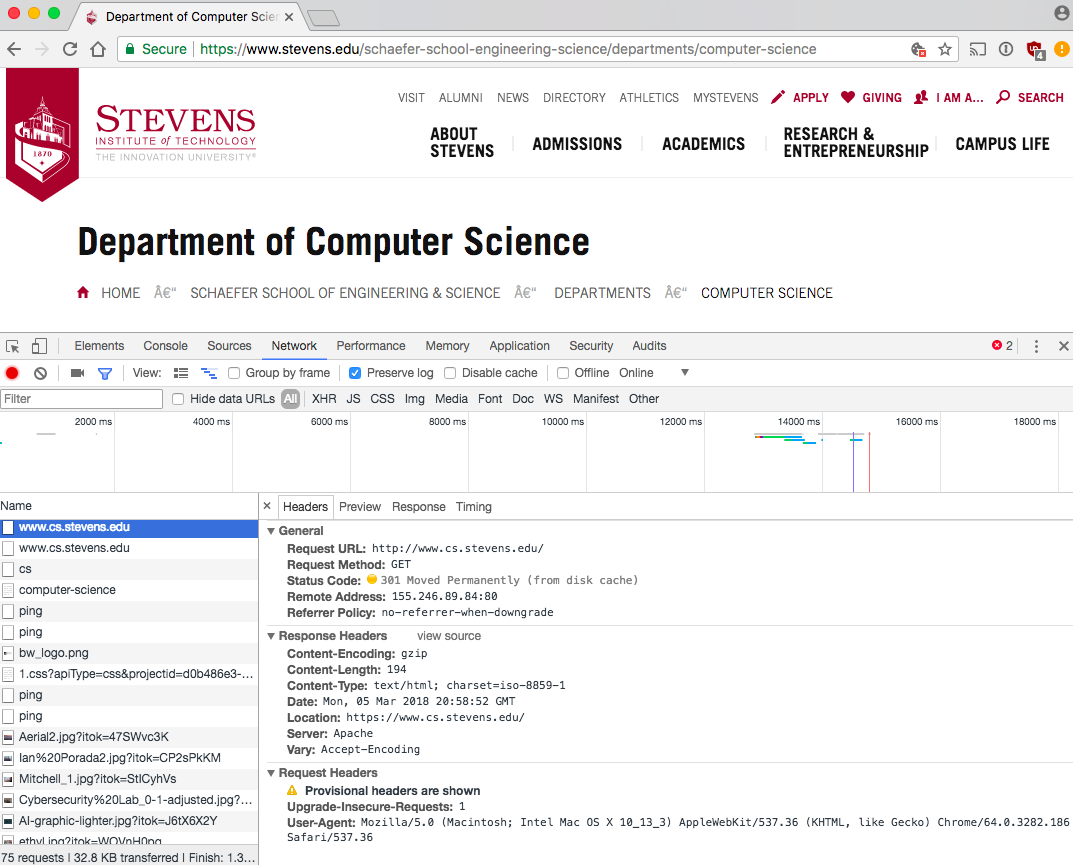
\includegraphics[scale=0.4]{pics/www.cs.stevens.edu.eps}
\end{center}


\subsection{HTTP - more than just text}
HTTP is a {\em Transfer Protocol} -- serving {\em data}, not any specific
text format.

\begin{itemize}
	\item {\tt Accept-Encoding} client header can specify different formats
		such as {\tt gzip} or {\tt deflate} for compression etc.
		communications, etc.
	\item corresponding server headers: {\tt Content-Type} and
		{\tt Content-Encoding}
\end{itemize}
\begin{center}
	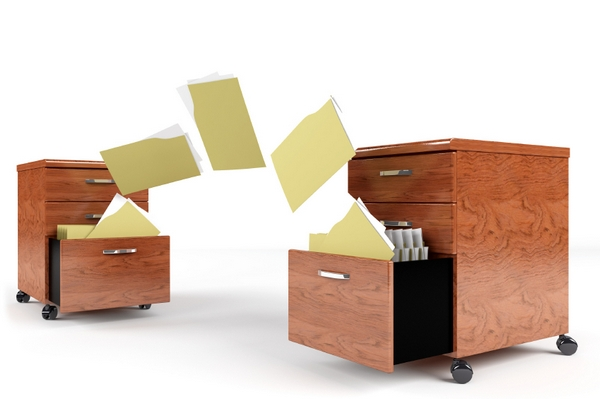
\includegraphics[scale=2.0]{pics/datatransfer.eps}
\end{center}

\subsection{HTTP - more than just static data}
HTTP is a {\em Transfer Protocol} -- what is transferred need not be
static; resources may generate different data to return based on many
variables.

\begin{itemize}
	\item CGI -- resource is {\em executed}, needs to generate
		appropriate response headers
	\item server-side scripting (ASP, PHP, Perl, ...)
	\item client-side scripting (JavaScript/ECMAScript/JScript,...)
	\item applications based on HTTP, using:
		\begin{itemize}
			\item AJAX
			\item RESTful services
			\item JSON, XML, YAML to represent state and
				abstract information
		\end{itemize}
\end{itemize}

\subsection{HTTP Proxy Servers}
\begin{itemize}
	\item HTTP traffic usually is very asymmetric
	\item a lot of the content is static
	\item network ACLs may restrict traffic flow
\end{itemize}
\vspace{.25in}
\begin{center}
	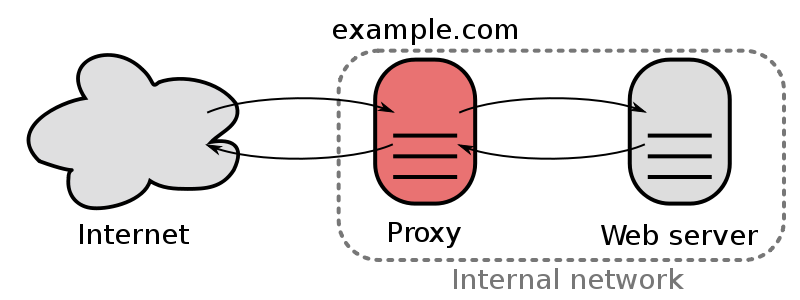
\includegraphics[scale=0.6]{pics/revproxy.eps}
\end{center}

\subsection{HTTP overload}
Ways to mitigate HTTP overload:

\begin{itemize}
	\item DNS round-robin to many web servers
	\item load balancing
	\item web cache / accelerators (reverse proxies)
	\item content delivery networks
\end{itemize}

These solutions depend on the location within the network and the scale of
the environment.

\subsection{Load Balancing}
\begin{center}
	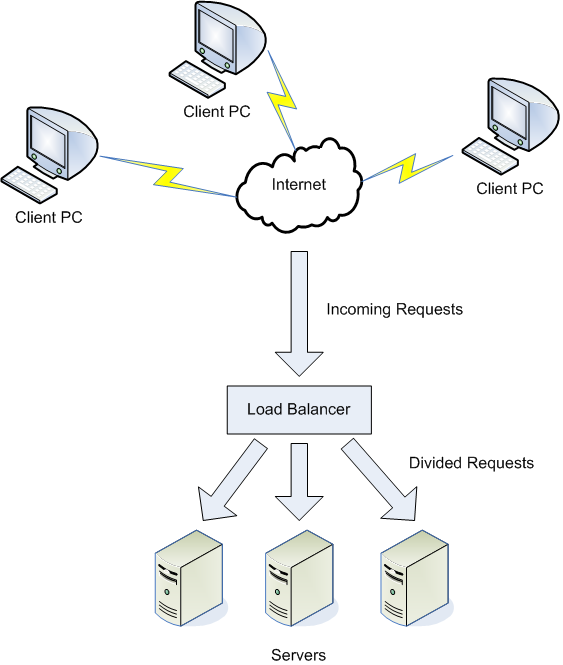
\includegraphics[scale=0.55]{pics/Lb101.eps}
\end{center}

\subsection{Load Balancing: Inbound}
\begin{center}
	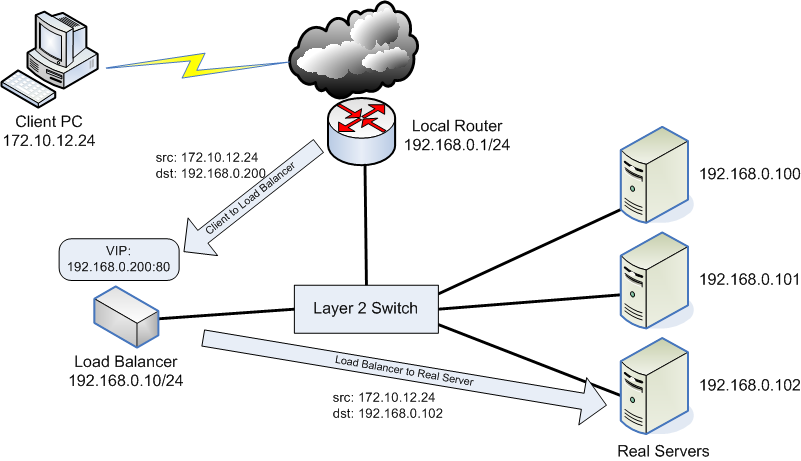
\includegraphics[scale=0.7]{pics/One-armed-inbound.eps}
\end{center}

\subsection{Load Balancing: Outbound}
\begin{center}
	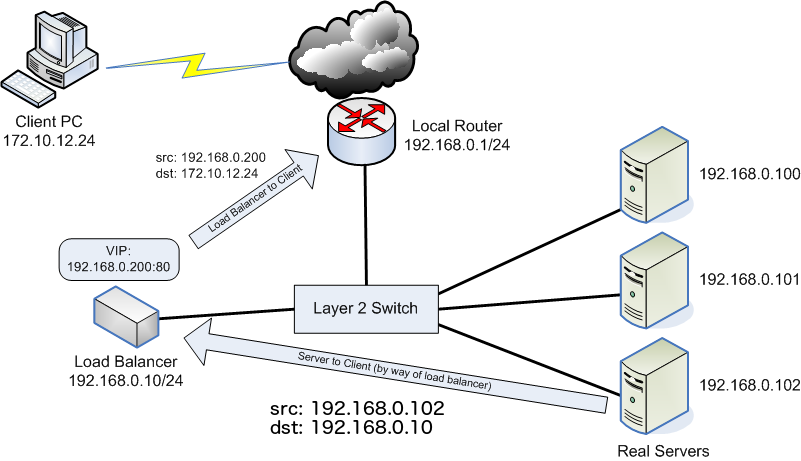
\includegraphics[scale=0.7]{pics/One-armed-outbound.eps}
\end{center}

\subsection{Load Balancing: Direct Server Return}
\begin{center}
	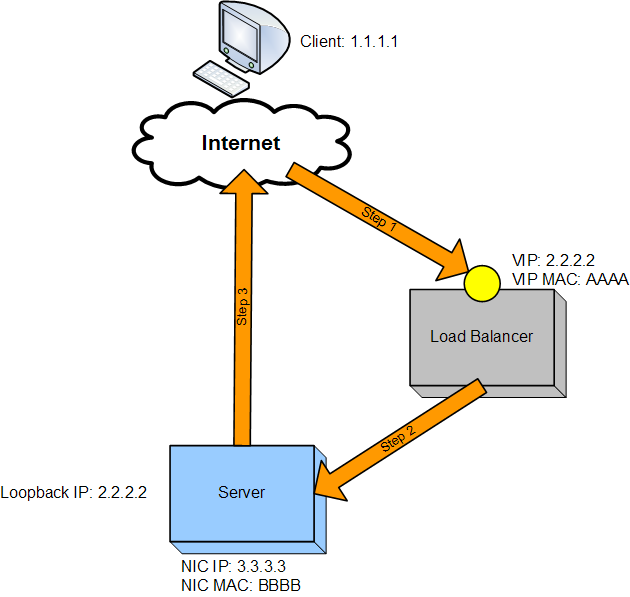
\includegraphics[scale=0.6]{pics/DSR.eps}
\end{center}

\subsection{Content Delivery Networks}
\begin{center}
	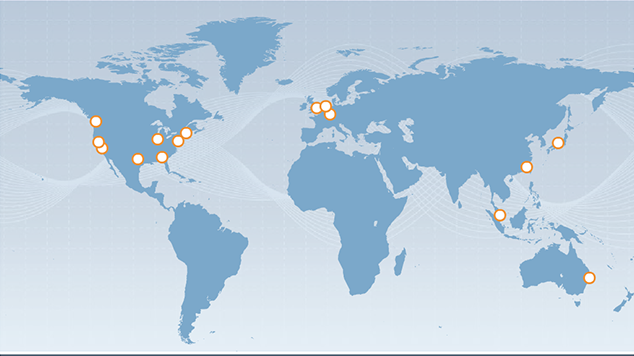
\includegraphics[scale=0.9]{pics/cdn.eps}
\end{center}

\subsection{Content Delivery Networks}
\begin{itemize}
	\item cache content in strategic locations
	\item determine location to serve from via geomapping of IP
		addresses (beware IPv6 aggregation!)
	\item often uses a separate domain to distinguish small
		objects/large objects or dynamic content/static content
	\item either out-sourced or in-house (if your organization is a
		Tier-1 or Tier-2 peering partner)
	\item request routing happens via Global Server Load Balancing,
		DNS-based request routing, anycasting etc.
	\item provides vast amounts of interesting data about your clients
		(see \verb+https://www.akamai.com/stateoftheinternet/+)
\end{itemize}

\subsection{CDN Implications}
\begin{itemize}
	\item your CDN sees all your traffic
	\item your CDN controls your TLS certificate keys
	\item your CDN is a multi-tenant environment
	\item your CDN may impose restrictions on your clients
	\item separation of cache-able content may
		require multiple (second-level) domains
\end{itemize}

\subsection{HTTP and DNS}
\vspace*{\fill}
\Huge
Both HTTP and DNS are trivial to set up. \\

Both HTTP and DNS are not trivial to get right. \\
\Normalsize
\vspace*{\fill}

\subsection{Reading}
HTTP etc.:
\begin{itemize}
	\item RFC 2616, 2818, 3875
	\item \verb+https://httpd.apache.org/docs/+
	\item \verb+https://www.w3.org/Protocols/+
	\item REST: \verb+https://is.gd/leSvGa+
	\item CDNs: \verb+https://is.gd/R5DoxA+
		\begin{itemize}
			\item \verb+https://www.edgecast.com/+
			\item \verb+https://aws.amazon.com/cloudfront/+
			\item \verb+https://www.akamai.com/+
			\item \verb+https://www.limelight.com/+
			\item ...
		\end{itemize}
	\item \verb+https://developer.yahoo.com/performance/rules.html+
\end{itemize}


\end{document}
